\section{Selecting and connecting qubits in an array}
\label{sec:platform-array-selection}

The gates above specify an operation on one spin or a chosen group
of spins. In an array, the applied electric and magnetic fields can
also reach other dots, and neighboring exchange couplings may
remain finite. \emph{Addressing} means making the intended qubit
or pair respond selectively to a control. Frequency separation,
spatially concentrated driving, and control of individual exchange
links provide complementary ways to do this.

\subsection{Selecting a spin by frequency and drive amplitude}

For approximately parallel local quantization axes, spin $i$ has
resonance frequency $\omega_i=g_i\mu_B B_i/\hbar$, with $B_i$ the
local static field magnitude and $g_i$ its effective $g$ factor.
A spatially varying static field can separate these frequencies.
A gate voltage can also shift a resonance by changing $g_i$ or the
electron's position in the field. Electrical tuning of the $g$
factor has been demonstrated in silicon quantum dots~\cite{Veldhorst2014Addressable}.
One can set the drive frequency to the target resonance, or tune
the target into resonance with a chosen drive frequency.

Suppose a constant pulse is resonant with spin $i$ and gives it
Rabi frequency $\Omega_i>0$. Its $\pi$-pulse time is
$\tau_\pi=\pi/\Omega_i$. If the same pulse drives another spin $j$
with Rabi frequency $\Omega_j$, that spin has detuning
$\Delta_j=\omega_j-\omega_i$. Neglecting exchange during this
single-spin pulse, Eq.~\eqref{eq:rabi-probability} gives
\begin{equation}
 P_{j,\mathrm{flip}}(\tau_\pi)
 =\frac{\Omega_j^2}{\Delta_j^2+\Omega_j^2}
   \sin^2\!\left(\frac{\tau_\pi}{2}
                   \sqrt{\Delta_j^2+\Omega_j^2}\right)
 \leq\frac{\Omega_j^2}{\Delta_j^2+\Omega_j^2}.
 \label{eq:platform-frequency-selection}
\end{equation}
Thus $|\Delta_j|\gg|\Omega_j|$ suppresses an unwanted flip
throughout the pulse. The resonance separation and the drive
strength induced on the spectator must be measured to choose a
drive frequency and amplitude that satisfy this condition
(Appendix~\ref{sec:processor-spectator-addressing}).
If both spins are resonant and appreciably
driven, frequency selection alone does not isolate the target.
For a fixed frequency separation, increasing the shared drive
amplitude to shorten a gate can reduce this selectivity.

Spatial control acts on the other quantity in this condition:
it reduces $\Omega_j$. With electric-dipole spin resonance, a
local gate can move the target electron more strongly than distant
electrons. The transverse magnetic-field gradient converts that
motion into a spin drive, as derived in
Eq.~\eqref{eq:micromagnet-rabi}. The longitudinal field variation
that separates resonance frequencies and the transverse gradient
that enables this drive have different roles, even when one
micromagnet provides both~\cite{Philips2022}. Electrical fields
extend beyond one dot, so locality must be assessed through the
resulting couplings rather than the electrode's name.

Suppressing spectator flips does not remove every action on its
state. A far-detuned drive also shifts the spectator's precession
frequency. Relative to an otherwise identical wait, it produces
an additional rotation $R_{z,j}(-\phi_j)$ with
\begin{equation}
 \phi_j\simeq\int_0^\tau\frac{\Omega_j(t)^2}{2\Delta_j}\,dt.
 \label{eq:platform-spectator-phase}
\end{equation}
This expression assumes fixed detuning, $|\Omega_j/\Delta_j|\ll1$,
and switching slow enough to follow the dressed eigenstates.
A spectator superposition can therefore acquire a phase even when
few flips occur. Measure the additional spectator phase produced by
the target pulse and include its reproducible part in the later
control reference (Appendix~\ref{sec:processor-spectator-addressing}).

\subsection{Selecting exchange links and parallel gates}

To select an exchange gate on neighboring dots, change their tunnel
barrier and, where needed, compensate the accompanying shifts of
the dot energies with other gate voltages. This changes the virtual
tunneling that produces $J$. In the four-dot chain of
Fig.~\ref{fig:platform-exchange-selection}, a gate on spins 2 and 3
requires a useful $J_{23}$ and sufficiently small unwanted actions
from $J_{12}$ and $J_{34}$ during the same interval. A residual
coupling of scale $J_{\mathrm{off}}$ acting for time $\tau$ has
exchange area of scale $J_{\mathrm{off}}\tau/\hbar$; the required
suppression therefore depends on gate duration and error tolerance.
Measure the selected and residual exchange couplings at the voltages
used for the complete layer. Adjust the barrier and compensating
plunger voltages so that the intended exchange areas reach their
targets while unwanted areas remain within the error allowance
(Appendix~\ref{sec:processor-parallel-exchange}).
Barrier control and compensation have been used to select
interactions in a silicon spin array~\cite{Philips2022}.

\begin{figure}[htbp]
 \centering
 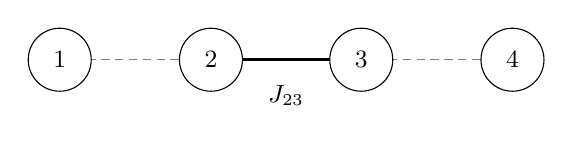
\begin{tikzpicture}[x=1.15cm,
   every node/.style={font=\small}]
  \draw[densely dashed,gray] (0,0)--(1.67,0);
  \draw[very thick] (1.67,0)--(3.33,0);
  \draw[densely dashed,gray] (3.33,0)--(5,0);
  \foreach \x/\lab in {0/1,1.67/2,3.33/3,5/4} {
   \node[draw,circle,fill=white,minimum size=8mm,inner sep=0pt]
     at (\x,0) {$\lab$};
  }
  \node[below] at (2.5,-0.2) {$J_{23}$};
 \end{tikzpicture}
 \caption{A four-dot exchange chain. The thick \(J_{23}\) link
 is selected for a gate on spins 2 and 3; the dashed links are
 available but intended to have small exchange during this pulse.
 Dots 1 and 3 have no direct exchange edge.}
 \label{fig:processor-four-dot-exchange}
 \label{fig:platform-exchange-selection}
\end{figure}
\FloatBarrier

The same chain shows when two pair gates can be independent during
one interval. Selecting $(1,2)$ and $(3,4)$ assigns each spin to
only one pair. If the coupling between the pairs is negligible,
their evolution factorizes:
\begin{equation}
 U_{12,34}=U_{12}\otimes U_{34}.
 \label{eq:platform-parallel-exchange}
\end{equation}
Selecting $(1,2)$ and $(2,3)$ instead makes spin 2 participate in
both interactions, generating a three-spin evolution that must be
designed as such. Exchange gates on edges with no shared spin are
therefore candidates for one parallel layer, provided unselected
couplings and spectator responses are also controlled.
Appendix~\ref{sec:processor-parallel-exchange} develops the resulting
scheduling conditions.

The physical exchange graph describes couplings between spins.
Its edges have different logical meanings for different encodings:
an internal edge of a three-spin block rotates one exchange-only
qubit, whereas an edge between blocks participates in a two-qubit
sequence. For two singlet--triplet blocks,
Eq.~\eqref{eq:st-capacitive-coupling} contributes a $Z_AZ_B$
interaction whenever $\kappa$ is nonzero, including during local
rotations. The same voltages can change both the local Hamiltonians
and $\kappa$. Independent logical gates therefore require the
unwanted interaction to be suppressed or refocused; otherwise the
full coupled evolution must be used. Appendix~\ref{sec:calibration-parallel-st-gates}
works through this control constraint.

\subsection{Acting on qubits without a direct link}

The four-dot graph has no exchange edge between sites 1 and 3.
One way to act on the states at those sites is to use a SWAP to
bring them onto an available edge. If $S_{23}$ exchanges the
states at sites 2 and 3 and $U_{12}$ is the desired operation
available on edge $(1,2)$, then
\begin{equation}
 U_{13}=S_{23}U_{12}S_{23}.
 \label{eq:platform-routed-gate}
\end{equation}
The rightmost SWAP brings the original state of site 3 to site 2,
and the leftmost restores the placement after the gate. This
identity holds for unknown or entangled inputs, because SWAP
permutes states without measuring them. Each dot remains occupied.
For an encoded qubit, swapping a single constituent spin generally
does not exchange the complete logical state; its logical
permutation must be constructed separately.
Appendix~\ref{sec:processor-swap-routing} develops SWAP routing
and the operations required along a longer path.

Shuttling provides another route by moving the electron itself
between dots. The transfer must avoid unwanted charge excitation
and spin flips, and the phase accumulated in the changing local
field must remain known or reproducible. The measured interdot
coupling and voltage-to-detuning response constrain the allowed
plunger-ramp speed, and the measured spin
phase sets the correction after transfer
(Appendix~\ref{sec:processor-shuttling}).
A shared quantum mode
can instead mediate an interaction while the electrons remain in
place; the useful interaction must compete with spin decoherence
and loss from the mode. The measured spin--mode couplings and loss
rates determine the usable detuning and interaction time
(Appendix~\ref{sec:processor-mode-coupling}).

The controls and detectors must also distinguish the intended
objects in an array. The measured voltage responses of the target
and affected neighbours determine the compensating electrode
changes needed to preserve their required energies and couplings
(Appendix~\ref{sec:processor-array-compensation}).
When several spins are read out, their converted charge
records must be distinguishable through the available sensors or
through measurements separated in time. Mean charge signals alone
do not specify joint outcome probabilities; correlations require
retaining the associated outcomes from each repetition.
Appendix~\ref{sec:processor-array-readout} develops the conditions
for separating those signals.
